\documentclass[a4paper,12pt]{article}

\usepackage[utf8]{inputenc}
\usepackage[spanish]{babel}
\usepackage{amsmath, amssymb}
\usepackage{graphicx}
\usepackage{float}
\usepackage{booktabs}
\usepackage{xcolor}
\usepackage{listings}
\usepackage{caption}
\usepackage{fancyhdr}
\usepackage{hyperref}
\usepackage{tikz}

\hypersetup{
    colorlinks=true,
    linkcolor=blue,
    urlcolor=blue,
    pdftitle={Práctica 0 - SPI UART PWM},
}

% === Definición de colores similares a Vivado ===
\definecolor{vivadoKeyword}{rgb}{0.6,0.0,0.6}
\definecolor{vivadoComment}{rgb}{0.0,0.5,0.0}
\definecolor{vivadoString}{rgb}{0.5,0.2,0.0}
\definecolor{vivadoBackground}{rgb}{0.97,0.97,0.97}

\lstdefinelanguage{VHDL}{
    morekeywords={library, use, entity, is, port, in, out, end, architecture, of, begin, signal, if, then, else, when, others, xor, and, or, not},
    sensitive=true,
    morecomment=[l]--,
    morestring=[b]",
}

\lstset{
    language=VHDL,
    backgroundcolor=\color{vivadoBackground},
    keywordstyle=\color{vivadoKeyword}\bfseries,
    commentstyle=\color{vivadoComment}\itshape,
    stringstyle=\color{vivadoString},
    basicstyle=\ttfamily\small,
    numbers=left,
    numberstyle=\tiny,
    numbersep=5pt,
    frame=single,
    breaklines=true,
    tabsize=2,
    captionpos=b
}

\title{Práctica N°0: Medicion de Corriente con ajuste de PWM visualizado mediante puerto UART}
\date{}

\begin{document}
\maketitle
\tableofcontents
\newpage


\section{Objetivos}

\subsection{Objetivo general}
Diseñar e implementar, desde cero en \textit{STM32CubeIDE}, un sistema que controle el \textit{duty cycle} de una señal \textbf{PWM}, lea la \textbf{corriente} mediante un sensor Hall y \textbf{visualice} las variables por \textbf{UART} usando PuTTY.

\subsection{Objetivos específicos}
\begin{enumerate}
  \item \textbf{Entorno y proyecto:} Crear el proyecto en \textit{STM32CubeIDE} y configurar reloj, pines y periféricos necesarios (TIMx para PWM, interfaz del sensor Hall, y USARTx para UART).
  \item \textbf{Mapeo de pines:} Asignar pines para la salida PWM, la interfaz del sensor Hall y la UART hacia el PC.
  \item \textbf{PWM:} Configurar TIMx en modo PWM con frecuencia adecuada (p.\,ej., $>20$\,kHz) y rango de \textit{duty cycle} 0\,\%–100\,\%.
  \item \textbf{Lectura de corriente:} Inicializar y leer el sensor Hall; convertir los datos crudos a unidades físicas (A) aplicando el factor de escala correspondiente.
  \item \textbf{Telemetría UART:} Transmitir por UART (p.\,ej., 115200\,bps) tramas legibles en PuTTY con \texttt{timestamp}, \texttt{duty\_cycle} e \texttt{I\_A}.
  \item \textbf{Validación:} Verificar en PuTTY que variaciones del \textit{duty} se reflejan en la corriente, adjuntando capturas de pantalla.
\end{enumerate}



\section{Desarrollo}

\subsection{Creación del Proyecto en STM32CubeIDE}

Para iniciar con la práctica es necesario crear un nuevo proyecto en el entorno \textbf{STM32CubeIDE}, el cual permite configurar los periféricos del microcontrolador y generar automáticamente el código base del proyecto.

\begin{enumerate}
    \item Abrir el programa \textbf{STM32CubeIDE}. Una vez cargada la interfaz, seleccionar la opción \textbf{File $\rightarrow$ New $\rightarrow$ STM32 Project}.  

    \begin{center}
        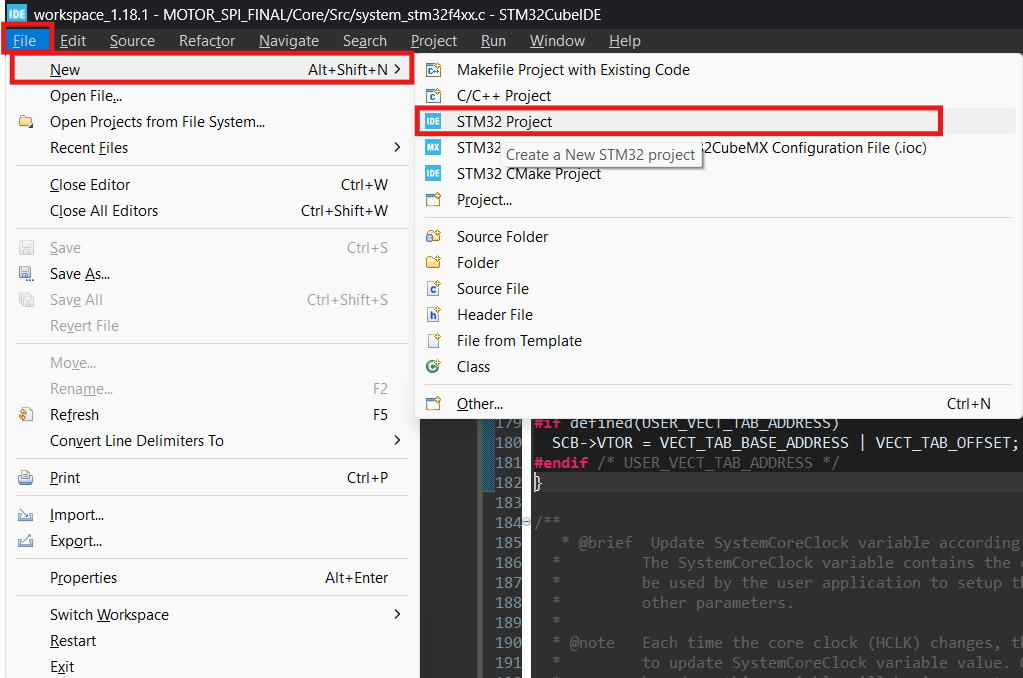
\includegraphics[width=0.8\textwidth]{Crear_proyecto/crear_stm32.png}
        \captionof{figure}{Selección de un nuevo proyecto en STM32CubeIDE.}
    \end{center}

    \item En la ventana emergente, seleccionar la tarjeta de desarrollo utilizada. Para esta práctica se emplea la \textbf{STM32F407G-DISC1}. Se puede buscar directamente por el nombre de la tarjeta en la pestaña \textbf{Board Selector}.  

    \begin{center}
        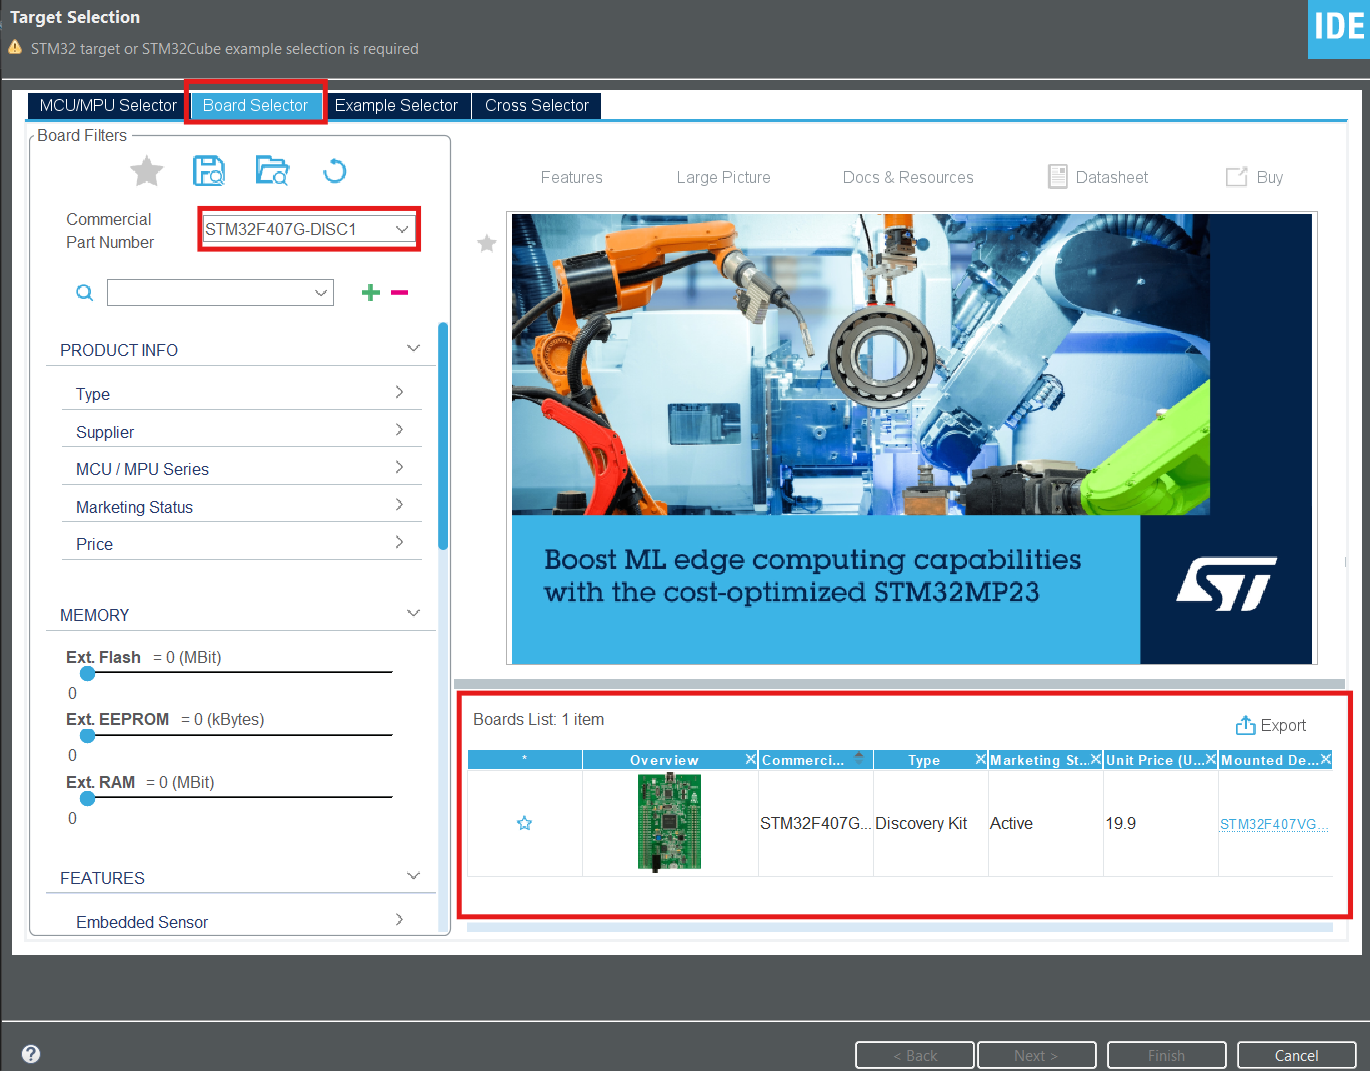
\includegraphics[width=0.8\textwidth]{Crear_proyecto/board_selector.png}
        \captionof{figure}{Selección de la tarjeta STM32F407G-DISC1 en el Board Selector.}
    \end{center}

    \item Asignar un nombre al proyecto y seleccionar la carpeta donde será guardado. Confirmar con \textbf{Finish}.  

    \begin{center}
        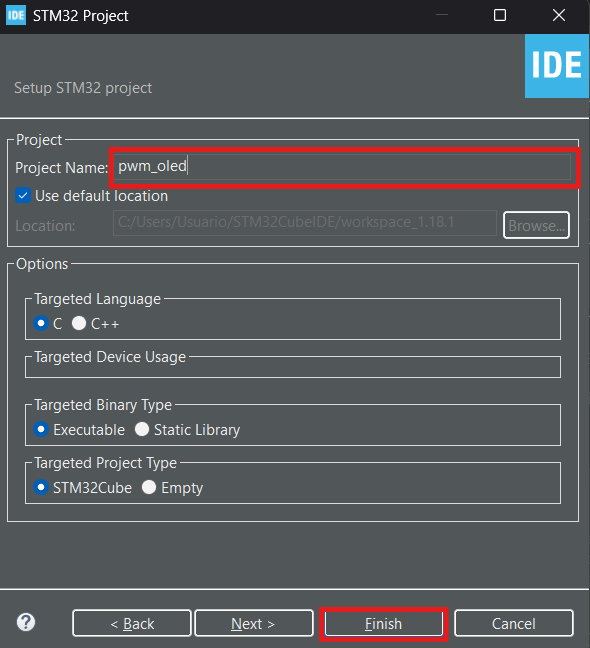
\includegraphics[width=0.8\textwidth]{Crear_proyecto/nombre_proyecto.png}
        \captionof{figure}{Asignación del nombre del proyecto.}
    \end{center}

    \item Una vez creado el proyecto, se abrirá automáticamente el archivo de configuración con extensión \textbf{.ioc}, que corresponde al \textbf{STM32CubeMX} integrado dentro de CubeIDE. Este archivo permite configurar los periféricos de manera gráfica.  

    \begin{center}
        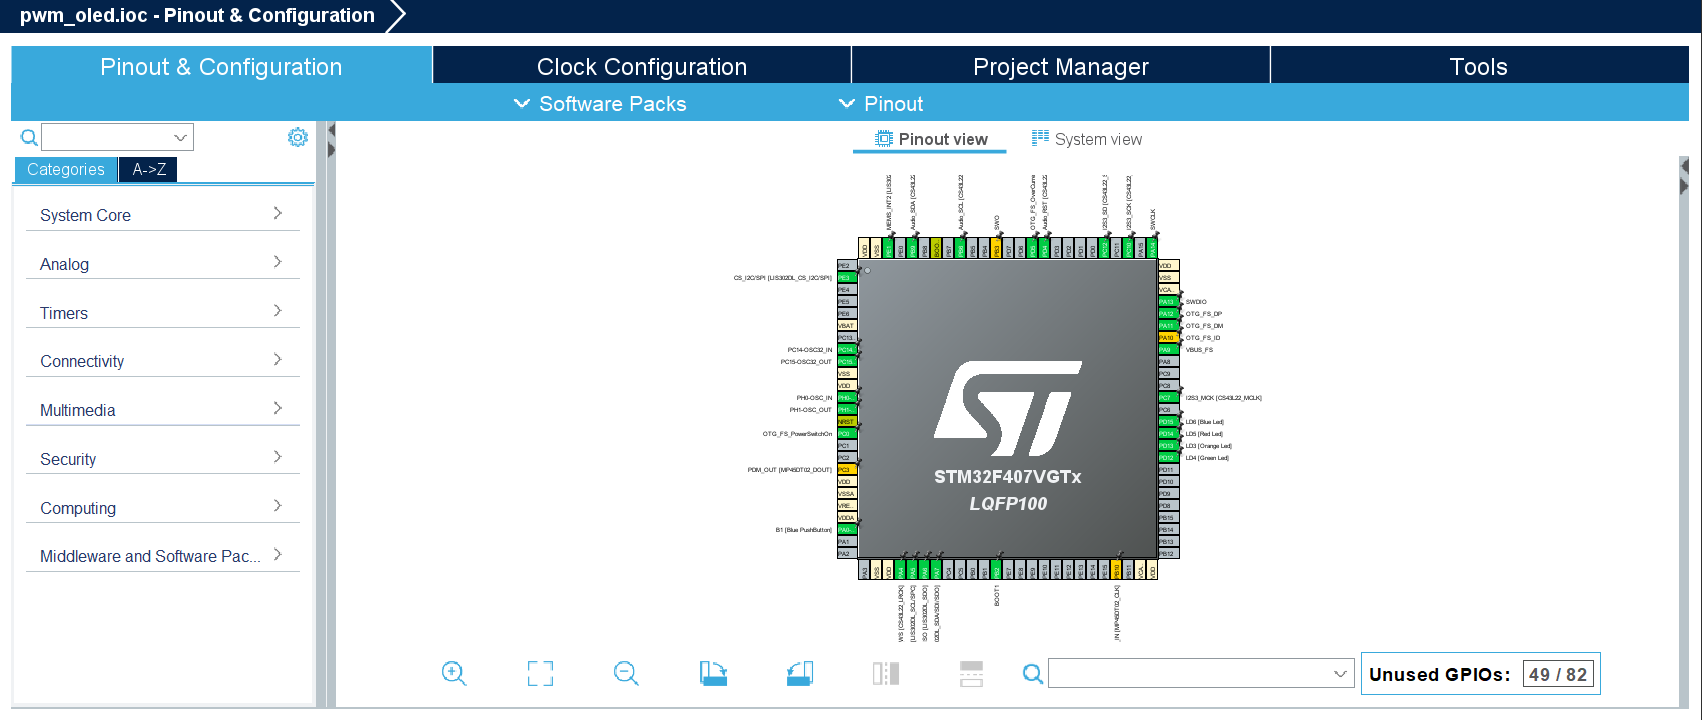
\includegraphics[width=0.8\textwidth]{Crear_proyecto/ioc.png}
        \captionof{figure}{Interfaz inicial del archivo \texttt{.ioc}.}
    \end{center}
\end{enumerate}

\section{Asignación de pines y configuración en STM32Cube}

\subsection{Resumen de pines (didáctico)}
\begin{table}[H]
\centering
\begin{tabular}{l l l p{6.5cm}}
\hline
\textbf{Señal} & \textbf{Función} & \textbf{Pin MCU} & \textbf{Motivo} \\
\hline
CS   & SPI NSS (sensor Hall) & \textbf{PB12} & NSS de \textbf{SPI2}; elección típica para selección de esclavo. \\
SCK  & SPI reloj              & \textbf{PB13} & \textbf{SPI2\_SCK}; facilita la configuración inicial. \\
SDO  & SPI MISO               & \textbf{PB14} & \textbf{SPI2\_MISO}; datos del sensor hacia el MCU. \\
PWM  & Salida PWM (TIMx\_CHy) & \textbf{PE13} & Canal PWM para accionar el driver (elegir TIM/CH compatibles). \\
IN1  & GPIO salida            & \textbf{PC2}  & Dirección/sentido de giro. \\
IN2  & GPIO salida            & \textbf{PE12} & Dirección/sentido de giro. \\
SLP  & GPIO salida            & \textbf{PE14} & \emph{Sleep/enable} del driver (activo según hoja de datos). \\
TX   & UART hacia PC          & \textbf{PA2}  & \textbf{USART2\_TX}; se mantiene para PuTTY. \\
RX   & UART desde PC          & \textbf{PA3}  & \textbf{USART2\_RX}; se mantiene para \textit{debug}. \\
\hline
\end{tabular}
\caption{Mapa de pines propuesto para SPI (sensor Hall), PWM (driver) y UART (telemetría).}
\end{table}

\subsection{Capturas del .ioc por lados del pinout}
% Reemplaza las rutas imgs/... con tus archivos de imagen
\begin{figure}[H]
\centering
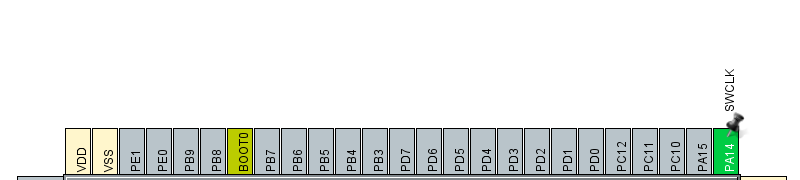
\includegraphics[width=0.88\linewidth]{ioc/norte.png}
\caption{Vista del \textit{Pinout} — \textbf{pines lado Norte}. Verificar presencia/ubicación de \textbf{PA2 (USART2\_TX)} y \textbf{PA3 (USART2\_RX)} según el mapeo de tu placa.}
\end{figure}

\begin{figure}[H]
\centering
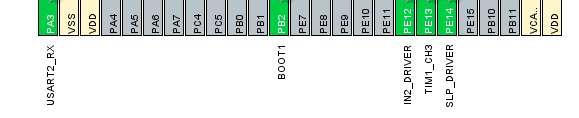
\includegraphics[width=0.88\linewidth]{ioc/sur.png}
\caption{Vista del \textit{Pinout} — \textbf{pines lado Sur}. Confirmar \textbf{PE12 (IN2)}, \textbf{PE13 (PWM)}, \textbf{PE14 (SLP)} en \textit{Alternate Function}/\textit{Output} según corresponda.}
\end{figure}

\begin{figure}[H]
\centering
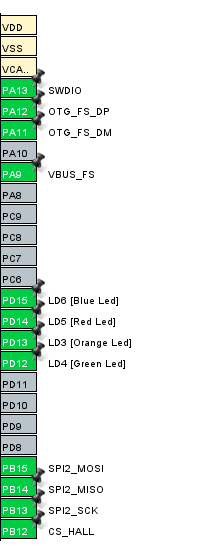
\includegraphics[angle=270,width=0.88\linewidth]{ioc/este.png}
\caption{Vista del \textit{Pinout} — \textbf{pines lado Este}. Revisar \textbf{PB12 (CS/NSS)}, \textbf{PB13 (SCK)}, \textbf{PB14 (SDO/MISO)} del bloque \textbf{SPI2}.}
\end{figure}

\begin{figure}[H]
\centering
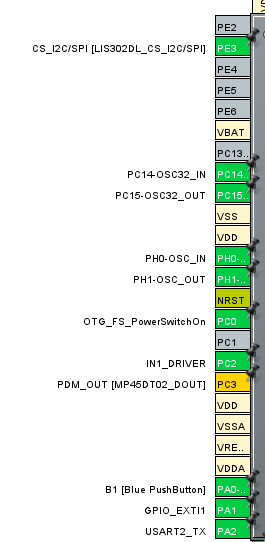
\includegraphics[angle=270,width=0.88\linewidth]{ioc/oeste.png}
\caption{Vista del \textit{Pinout} — \textbf{pines lado Oeste}. }
\end{figure}

\subsection{Capturas específicas por periférico}
\begin{figure}[H]
\centering
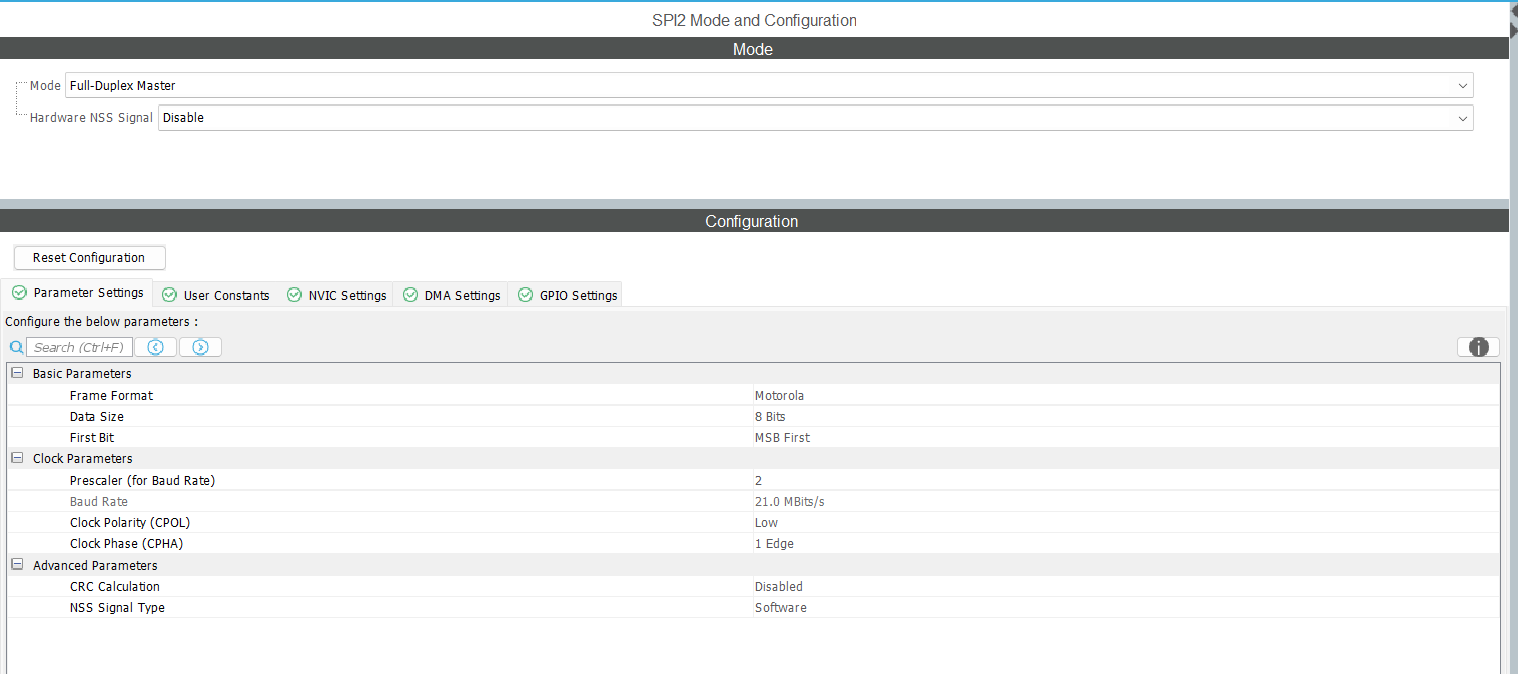
\includegraphics[width=0.88\linewidth]{Perifericos/spi2.png}
\caption{\textbf{SPI2} configurado con \textbf{PB12 (NSS)}, \textbf{PB13 (SCK)}, \textbf{PB14 (MISO)} .}
\end{figure}

\begin{figure}[H]
\centering
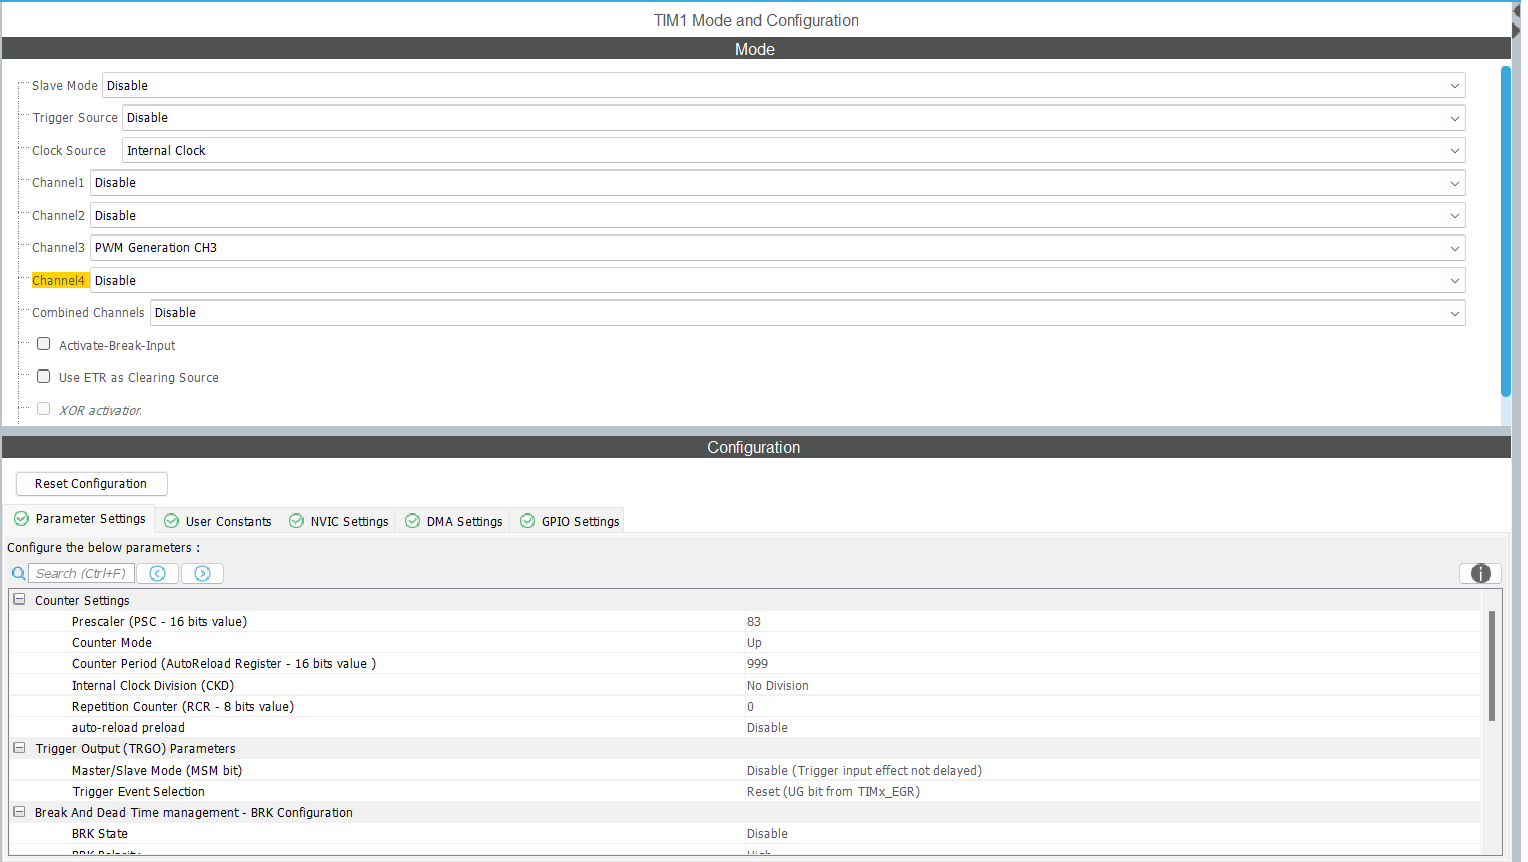
\includegraphics[width=0.88\linewidth]{Perifericos/tim1.png}
\caption{\textbf{PWM} en \textbf{PE13} (TIMx\_CHy) .}
\end{figure}

\begin{figure}[H]
\centering
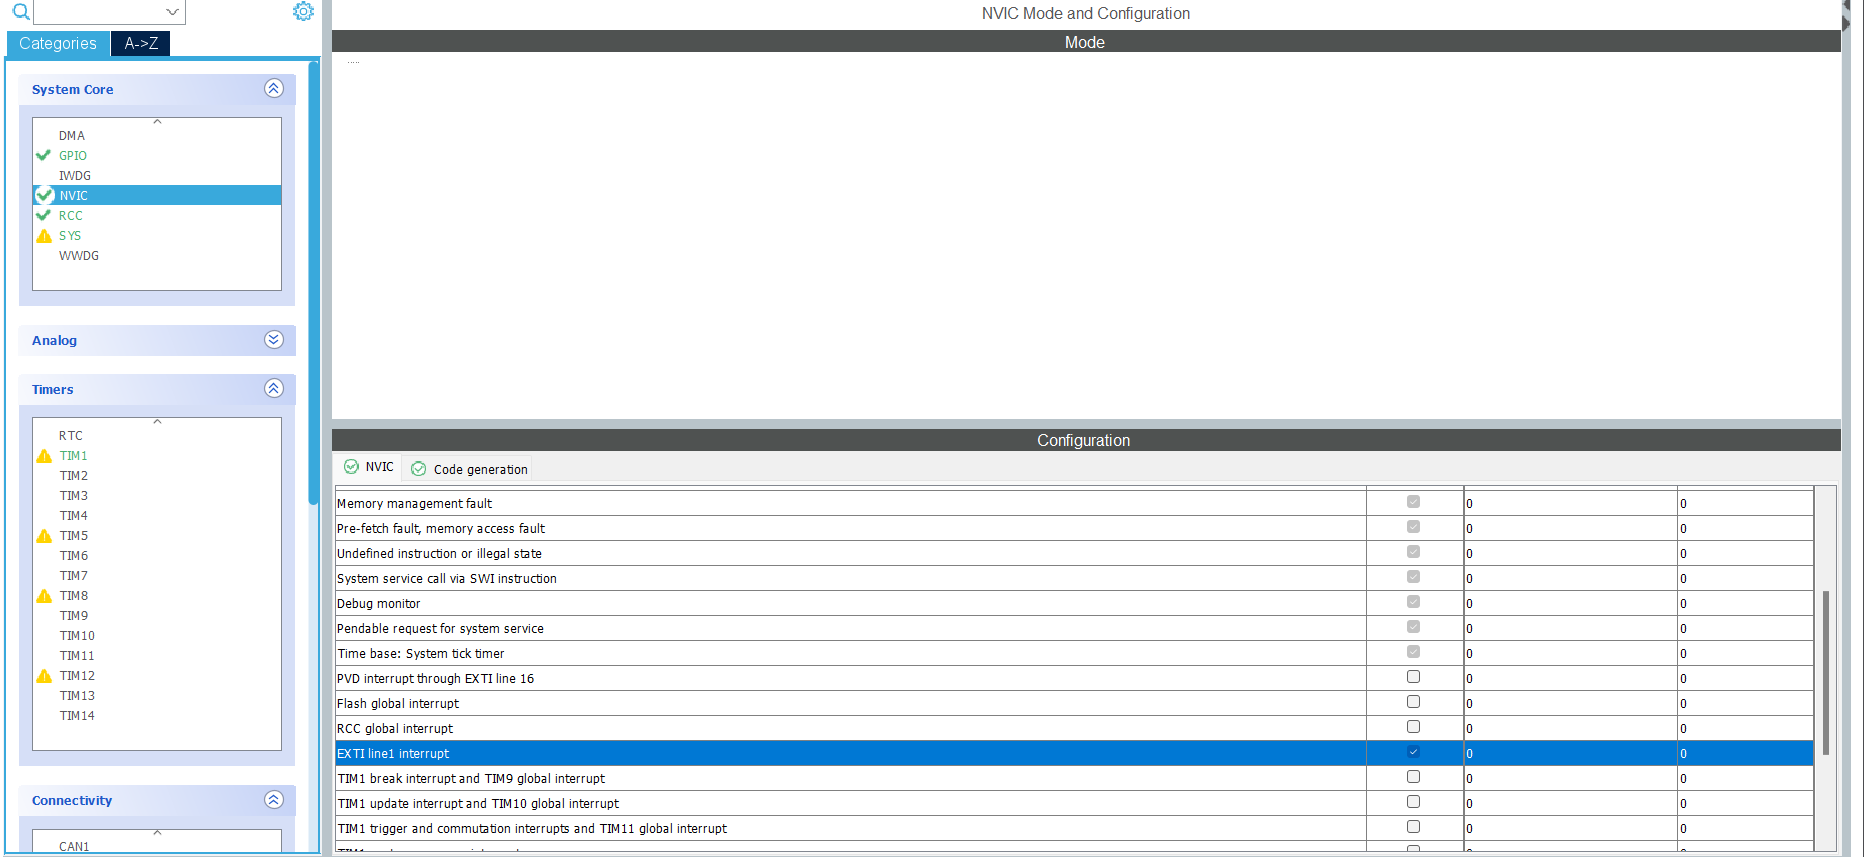
\includegraphics[width=0.88\linewidth]{Perifericos/interrupciones.png}
\caption{Habilitación de Interrupciones en el pin del pulsante.}
\end{figure}

\begin{figure}[H]
\centering
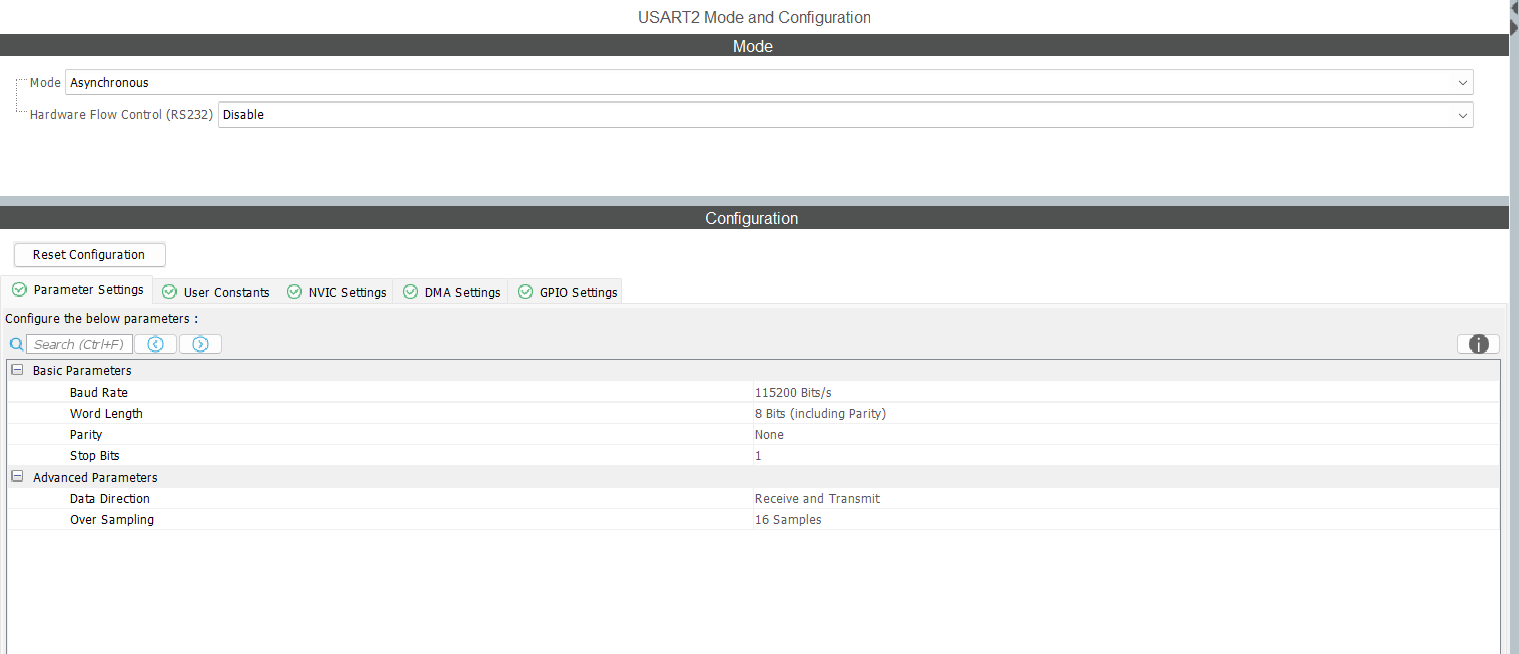
\includegraphics[width=0.88\linewidth]{Perifericos/uart2.png}
\caption{\textbf{USART2} en \textbf{PA2/PA3}}
\end{figure}





\subsection{Ubicación segura del código en STM32CubeIDE}

Al trabajar con proyectos generados desde STM32CubeMX, es importante conocer en qué partes del código se deben realizar las modificaciones para evitar que se borren cuando el proyecto se regenere.  

El código que genera automáticamente STM32CubeMX incluye secciones delimitadas por comentarios especiales. Las zonas seguras para agregar código personalizado están indicadas de la siguiente manera:  

\begin{lstlisting}[language=C, caption={Secciones seguras en el archivo \texttt{main.c}}]
/* USER CODE BEGIN 0 */
// Aqui se puede colocar codigo global (variables, librerias externas, etc.)
/* USER CODE END 0 */

int main(void)
{
  /* USER CODE BEGIN 1 */
  // Codigo antes de la inicializacion de perifericos
  /* USER CODE END 1 */

  /* USER CODE BEGIN 2 */
  // Codigo despues de la inicializacion de perifericos
  /* USER CODE END 2 */

  while (1)
  {
    /* USER CODE BEGIN WHILE */
    // Codigo dentro del bucle principal
    /* USER CODE END WHILE */

    /* USER CODE BEGIN 3 */
    // Codigo adicional dentro del bucle principal
    /* USER CODE END 3 */
  }
}
\end{lstlisting}

De igual forma, en los archivos de interrupciones (\texttt{stm32f4xx\_it.c}) y en otros módulos del proyecto, siempre aparecerán las mismas etiquetas:  

\begin{lstlisting}[language=C, caption={Ejemplo de secciones seguras en interrupciones}]
/* USER CODE BEGIN  */
// Codigo del estudiante
/* USER CODE END  */
\end{lstlisting}

\textbf{Regla importante:}  
\begin{itemize}
    \item Todo el código del estudiante (funciones, variables, configuraciones adicionales) debe ir únicamente dentro de las secciones delimitadas por \texttt{USER CODE BEGIN} y \texttt{USER CODE END}.
    \item Nunca se debe modificar el código fuera de esas áreas, ya que será sobrescrito automáticamente cuando se regenere el proyecto desde STM32CubeMX.
\end{itemize}

Esto garantiza que los cambios del estudiante permanezcan intactos incluso si se reconfiguran los periféricos o se actualiza el archivo \texttt{.ioc}.


\section{Estructura del archivo \texttt{main.c}}

A continuación se presenta una explicación por secciones del fichero \texttt{main.c} suministrado. Está pensada para un estudiante que se inicia en STM32CubeIDE/STM32CubeMX: cada bloque muestra el código relevante dentro de un entorno \texttt{lstlisting} y una explicación clara y concisa.

\subsection{Encabezado e inclusiones}
\begin{lstlisting}[language=C]
/* Includes --*/
#include "main.h"
#include "usb_host.h"
#include <stdio.h>
\end{lstlisting}

Explicación: \texttt{main.h} contiene las definiciones generadas por CubeMX (pines, prototipos). \texttt{usb\_host.h} es el middleware para el host USB. \texttt{stdio.h} se incluye para usar \texttt{printf} redirigido vía UART (ver \texttt{\_\_io\_putchar}).

\subsection{Definiciones de pines (macros)}
\begin{lstlisting}[language=C]
#define CS_HALL_Pin        GPIO_PIN_12
#define CS_HALL_GPIO_Port  GPIOB
#define IN1_DRIVER_Pin        GPIO_PIN_2
#define IN1_DRIVER_GPIO_Port  GPIOC
#define IN2_DRIVER_Pin        GPIO_PIN_12
#define IN2_DRIVER_GPIO_Port  GPIOE
#define SLP_DRIVER_Pin        GPIO_PIN_14
#define SLP_DRIVER_GPIO_Port  GPIOE
\end{lstlisting}

Explicación: CubeMX genera macros para acceder a pines por nombre legible. Usar estas macros evita escribir directamente números de pin/puerto y hace el código más mantenible.

\subsection{Handles de periféricos}
\begin{lstlisting}[language=C]
SPI_HandleTypeDef hspi2;
TIM_HandleTypeDef htim1;
UART_HandleTypeDef huart2;
\end{lstlisting}

Estos objetos ("handles") mantienen el estado y la configuración de cada periférico (SPI2, TIM1, USART2). Son inicializados por las funciones \texttt{MX\_*\_Init()} generadas por CubeMX.

\subsection{Prototipos y funciones inline auxiliares}
\begin{lstlisting}[language=C]
static inline void driver_enable(uint8_t en) {
HAL_GPIO_WritePin(SLP_DRIVER_GPIO_Port, SLP_DRIVER_Pin, en ? GPIO_PIN_SET : GPIO_PIN_RESET);
}

typedef enum { DIR_ADELANTE = 0, DIR_ATRAS = 1 } dir_t;
static inline void driver_set_dir(dir_t d) { ... }
\end{lstlisting}

Explicación: funciones \texttt{inline} pequeñas para controlar el driver (activar/desactivar sleep y seleccionar dirección). Usar \texttt{HAL\_GPIO\_WritePin} es la forma HAL de cambiar pines.

\subsection{Variables de usuario y tabla de pasos PWM}
\begin{lstlisting}[language=C]
uint32_t last_press_time = 0;  // Antirrebote
volatile uint8_t step_count = 0;
const uint8_t duty_steps[6] = {0, 20, 40, 60, 80, 90};
\end{lstlisting}

\texttt{last\_press\_time} guarda el tiempo del último pulso para debouncing. \texttt{step\_count} es \texttt{volatile} porque puede cambiar en una ISR. \texttt{duty\_steps} define los porcentajes de duty cycle predefinidos.

\subsection{Función para ajustar PWM}
\begin{lstlisting}[language=C]
void Set_PWM_Duty(uint8_t percent) {
if (percent > 100) return;
uint32_t pulse = (percent * (__HAL_TIM_GET_AUTORELOAD(&htim1) + 1)) / 100;
__HAL_TIM_SET_COMPARE(&htim1, TIM_CHANNEL_3, pulse);
}
\end{lstlisting}

Explicación: calcula el valor del "compare" a partir del autoreload del temporizador (ARR) para obtener el duty en porcentaje. Esto permite cambiar el ciclo de trabajo sin tocar la configuración del temporizador.

\subsection{Manejador de interrupción externa (botón)}
\begin{lstlisting}[language=C]
void HAL_GPIO_EXTI_Callback(uint16_t GPIO_Pin) {
if (GPIO_Pin == GPIO_PIN_1) {
if (HAL_GetTick() - last_press_time > 50) {
step_count = (step_count + 1) % 6;
Set_PWM_Duty(duty_steps[step_count]);
last_press_time = HAL_GetTick();
}
}
}
\end{lstlisting}

Explicación: esta es la "callback" HAL para interrupciones por GPIO (configurada en \texttt{MX\_GPIO\_Init}). Usa \texttt{HAL\_GetTick()} para antirrebote y avanza al siguiente paso de duty cycle.

\newpage

\subsection{Lectura SPI del sensor de corriente}
\begin{lstlisting}[language=C]
uint16_t Read_Current_Raw(void) {
uint8_t tx_dummy[2] = {0x00, 0x00};
uint8_t rx_data[2] = {0};
HAL_GPIO_WritePin(GPIOB, GPIO_PIN_12, GPIO_PIN_RESET); // CS low
HAL_SPI_TransmitReceive(&hspi2, tx_dummy, rx_data, 2, HAL_MAX_DELAY);
HAL_GPIO_WritePin(GPIOB, GPIO_PIN_12, GPIO_PIN_SET); // CS high
uint16_t raw = ((uint16_t)rx_data[0] << 8) | rx_data[1];
return raw & 0x0FFF;  // 12 bits
}
\end{lstlisting}

Explicación: protocolo SPI típico: bajar CS, intercambiar bytes, subir CS. El valor leído se empaqueta y se limita a 12 bits.

\subsection{Redirección de printf a UART}
\begin{lstlisting}[language=C]
int __io_putchar(int ch) {
HAL_UART_Transmit(&huart2, (uint8_t *)&ch, 1, HAL_MAX_DELAY);
return ch;
}
\end{lstlisting}

Nota: esta función permite usar \texttt{printf} en el firmware (depende del retargeting de la librería estándar en su proyecto).

\subsection{Función \texttt{main} y bucle principal}
\begin{lstlisting}[language=C]
int main(void) {
HAL_Init();
SystemClock_Config();
MX_GPIO_Init();
MX_USB_HOST_Init();
MX_SPI2_Init();
MX_TIM1_Init();
MX_USART2_UART_Init();
driver_enable(1);
driver_set_dir(DIR_ADELANTE);
HAL_TIM_PWM_Start(&htim1, TIM_CHANNEL_3);
Set_PWM_Duty(0);
while (1) {
MX_USB_HOST_Process();
// toma 10 muestras espaciadas y calcula promedio
// calcula corriente en mA y la imprime
// aumenta PWM si la corriente excede un umbral
HAL_Delay(1000);
}
}
\end{lstlisting}

Explicación: el flujo típico generado por CubeMX: inicializar HAL, configurar reloj, inicializar periféricos (las funciones \texttt{MX\_*\_Init} son generadas automáticamente). Después viene la inicialización específica del usuario (activar driver, iniciar PWM) y el bucle infinito donde se leen sensores, se procesan datos y se toman decisiones.

\subsection{Inicialización de periféricos (MX\_*\_Init)}
\begin{lstlisting}[language=C]
static void MX_TIM1_Init(void) { ... }
static void MX_SPI2_Init(void) { ... }
static void MX_USART2_UART_Init(void) { ... }
static void MX_GPIO_Init(void) { ... }
\end{lstlisting}

Estos bloques contienen la configuración detallada (prescaler, periodo, polaridades, modos SPI/UART, configuración de pines). Si modificas parámetros en CubeMX, estas funciones son reescritas, por eso las secciones de usuario están delimitadas con \texttt{/* USER CODE BEGIN */} / \texttt{END} para preservar cambios manuales.



\section{Carga del Programa en la Placa}

Una vez configurados los periféricos y desarrollado el código fuente, el siguiente paso es \textbf{cargar el programa en la placa STM32F407G-DISC1}. Para ello, el entorno de desarrollo \textbf{STM32CubeIDE} ofrece un flujo de compilación, depuración y carga que debe seguirse de manera ordenada:

\begin{enumerate}
    \item \textbf{Compilación del proyecto}: se realiza utilizando el icono del \textbf{martillo} ubicado en la barra de herramientas. Este paso genera los archivos binarios y permite verificar si existen errores de sintaxis o configuración.
    
    \begin{figure}[H]
        \centering
        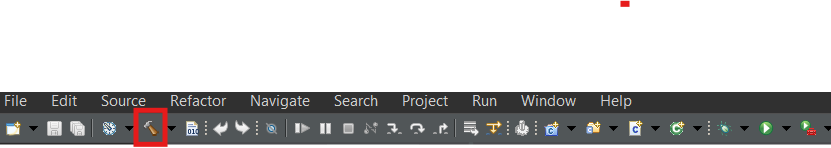
\includegraphics[width=0.9\textwidth]{Carga_en_placa/martillo.png}
        \caption{Icono de Compilación del proyecto mediante el icono del martillo.}
        \label{fig:compilacion_martillo}
    \end{figure}

    \item \textbf{Depuración inicial (Debug Communication)}: en este paso se utiliza el icono con forma de \textbf{cucaracha}, que inicia la depuración y establece la comunicación con la placa. Aquí se pueden detectar errores relacionados con la conexión o la carga del firmware.  
    
    \begin{figure}[H]
        \centering
        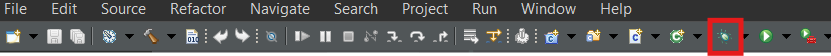
\includegraphics[width=0.9\textwidth]{Carga_en_placa/cucaracha.png}
        \caption{Iconon de Depuración inicial con el icono de la cucaracha en STM32CubeIDE.}
        \label{fig:debug_cucaracha}
    \end{figure}

    \item \textbf{Carga final del programa}: si no se presentan errores en los pasos anteriores, el programa es transferido a la memoria del microcontrolador. Una vez cargado, la placa ejecutará automáticamente el código y se podrán observar los resultados directamente en el hardware.
    
    \begin{figure}[H]
        \centering
        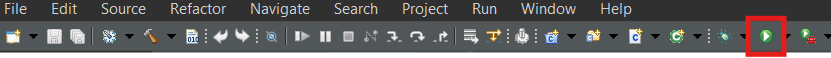
\includegraphics[width=0.9\textwidth]{Carga_en_placa/subir.png}
        \caption{Icono de carga del programa en la placa STM32F407G-DISC1.}
        \label{fig:carga_programa}
    \end{figure}
\end{enumerate}




\section{Resultados}

Durante la ejecución del programa, el sistema permitió el control del motor mediante el ajuste del ciclo útil de la señal PWM y la visualización simultánea de la corriente medida en la pantalla OLED. En la Figura~\ref{fig:resultado} se muestra una captura de pantalla del funcionamiento correcto del sistema, donde se observa la lectura de la corriente proveniente del sensor TLI4970 y la variación del valor al modificar el ciclo útil con los pulsadores.

\begin{figure}[H]
\centering
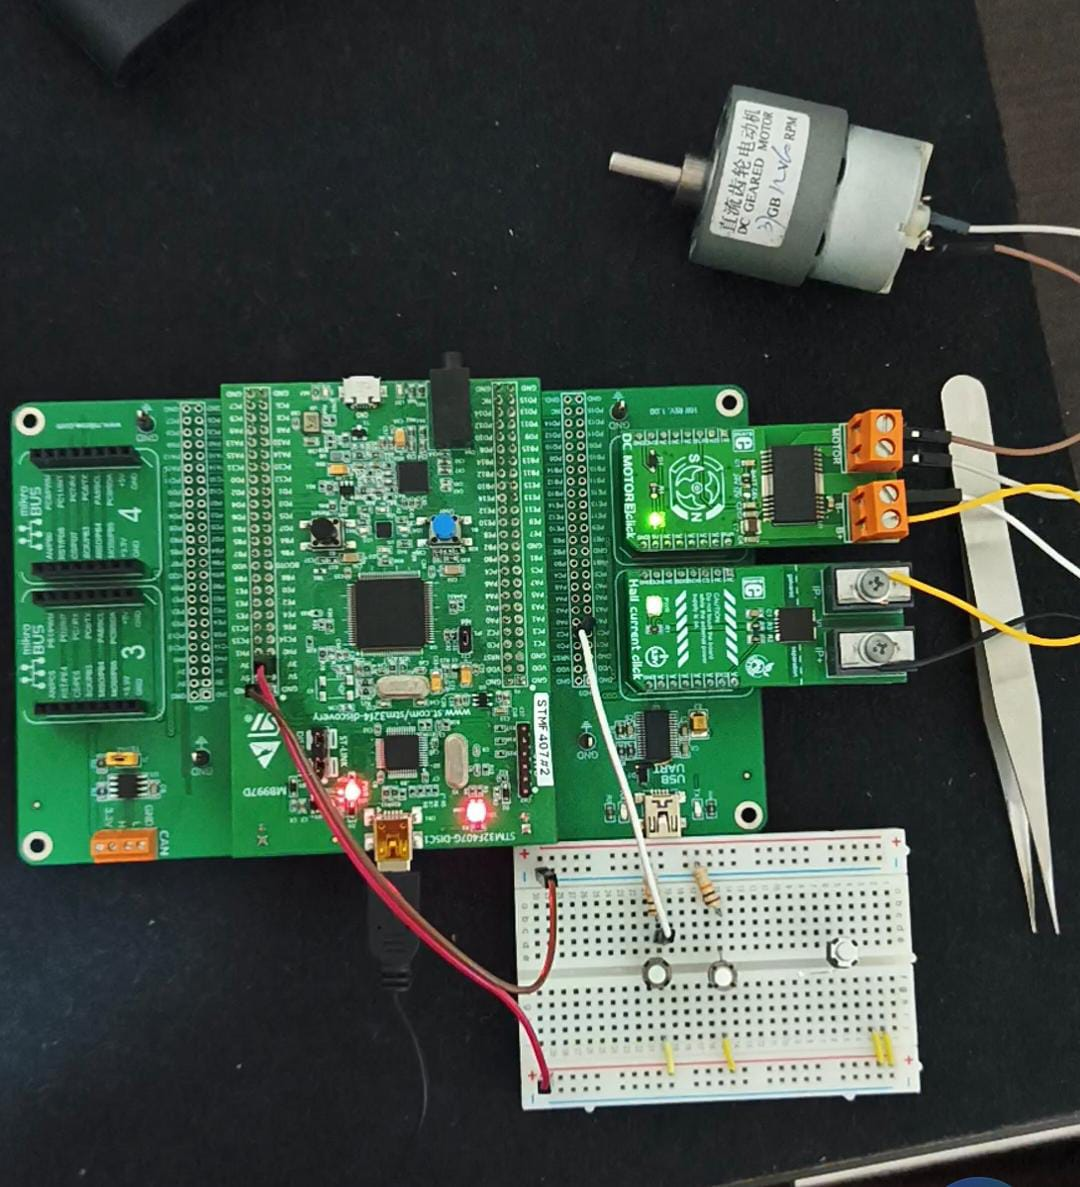
\includegraphics[width=0.7\textwidth]{Resultados/result_motor.jpg}
\caption{Funcionamiento del sistema mostrando la lectura de corriente y el control PWM.}
\label{fig:resultado}
\end{figure}

El sistema responde de forma estable y coherente con los cambios de control, validando la correcta integración de los periféricos SPI, PWM, UART y las interrupciones externas implementadas en el archivo \texttt{main.c}.

\begin{figure}[H]
\centering
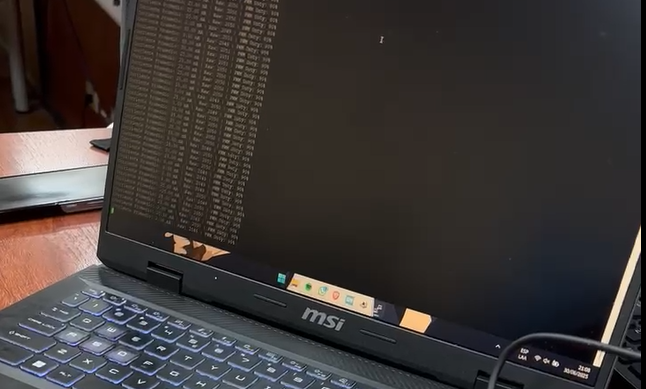
\includegraphics[width=0.7\textwidth]{Resultados/Registro pwm.png}
\caption{Funcionamiento del sistema mostrando la lectura de corriente y el control PWM.}
\label{fig:resultado}
\end{figure}

\end{document}
